\chapter{Introduction}

\section{Motivation}
Carbonaceous nanoparticles, such as Carbon Black (CB) and soot, are widely encountered in nature and engineering. Every year, nearly 9.5 megatons of soot (black carbon) is emitted into the atmosphere from anthropogenic activities and natrual sources such as wildfires and volcanoes~\citep{myhre2014anthropogenic}. The wide light absorption range of soot reduces the albedo of snow-covered area and alters the radiative forcing balance in the atmosphere making soot the third strongest contributor to climate change after methane and carbon dioxide~\citep{myhre2014anthropogenic}. Also, exposure to combustion-generated soot could promote respiratory and cardiovascular disease~\citep{world2013health}. So, strict regulations are targeting combustion engines to limit environmental and health risks from soot formation~\citep{integrated2019}. Accurate and affordable models are essential for the prediction of soot composition and morphology in combustion devices and help to reduce the emissions in engines. They can also provide better understanding of soot optical properties that are major indicator of soot environmental effects.

On the other hand, CB with a similar synthesis process and structure to soot but higher elemental carbon to hydrogen ratios ($>$97\%)~\citep{watson2001carbon} is commercially produced and sold in large scales. In fact, CB is the largest industrially produced nanomaterial by value and volume ($\sim$15 megatons per year with a value of \$17B) with applications as a reinforcing agent in rubber and tire industries~\citep{international2016carbon} and conductive additive in lithium-ion batteries~\citep{Palomares2010}. CB is primarily manufactured by the so-called furnace process where about 50\% of heavy fuel oil is partially combusted to convert the rest of it into CB~\citep{pratsinis2011history}. This process suffers from low mass yield and excessive emission, generating 4 tons of $\mathrm{CO_2}$ per each ton of product on average~\citep{bansal1993carbon}. Plasma reactor is an emerging alternative production method with distinct advantages over flame-based methods: They can achieve 100\% carbon yields with no direct $\mathrm{CO_2}$ emission or other pollutants~\citep{cho2004conversion}, and the energy required for pyrolysis is supplied by an electric arc that does not depend on the feedstock composition. Controlling CB properties such as its specific surface area (or primary particle diameter), hard agglomerate size (or gyration diameter of agglomerates with primary particles connected to each other by strong chemical bonds), and composition (or particle carbon to hydrogen ratio) is important to make process economical and to achieve specific grades of CB for different target applications. However, this is a challenging task because of the complexity of CB formation and mass growth processes and its coupling with gas phase chemistry, dependence on local temperature and pressure. This requires accurate process design and optimization tools that provides insight into CB formation and evolution process, and inform manufacturer's decisions to adjust to produce CB with desired grades~\citep{park2005influence}.
 
The term \textit{"soot}" usually refers to unwanted particulate matter formed during incomplete combustion of any carbon-containing material from jet and diesel fuel to wood, heavy oil, and plastics with variable organic content and large H/C ratios~\citep{watson2001carbon}, but this research focuses on soot particles generated under controlled laboratory conditions from fuels with known compositions. The mature soot formed in methane and ethylene premixed flame can reach 95\% elemental C/H ratio~\cite{russo2015dehydrogenation}, which is close to CB composition. The comparison of transmission electron microscopy (TEM) images of industrially produced CB~\citep{singh2018nanostructure} with soot sampled from diesel fuel~\citep{vander2007hrtem, lapuerta2017morphological} shown in Fig.\ref{fig:sootCBHRTEM} indicates similarity of their morphology and structure. Hereafter, soot is used to describe carbonaceous nanoparticels produced in flame/reactor during combustion/pyrolysis.

\begin{figure}[!htbp]
	\centering
	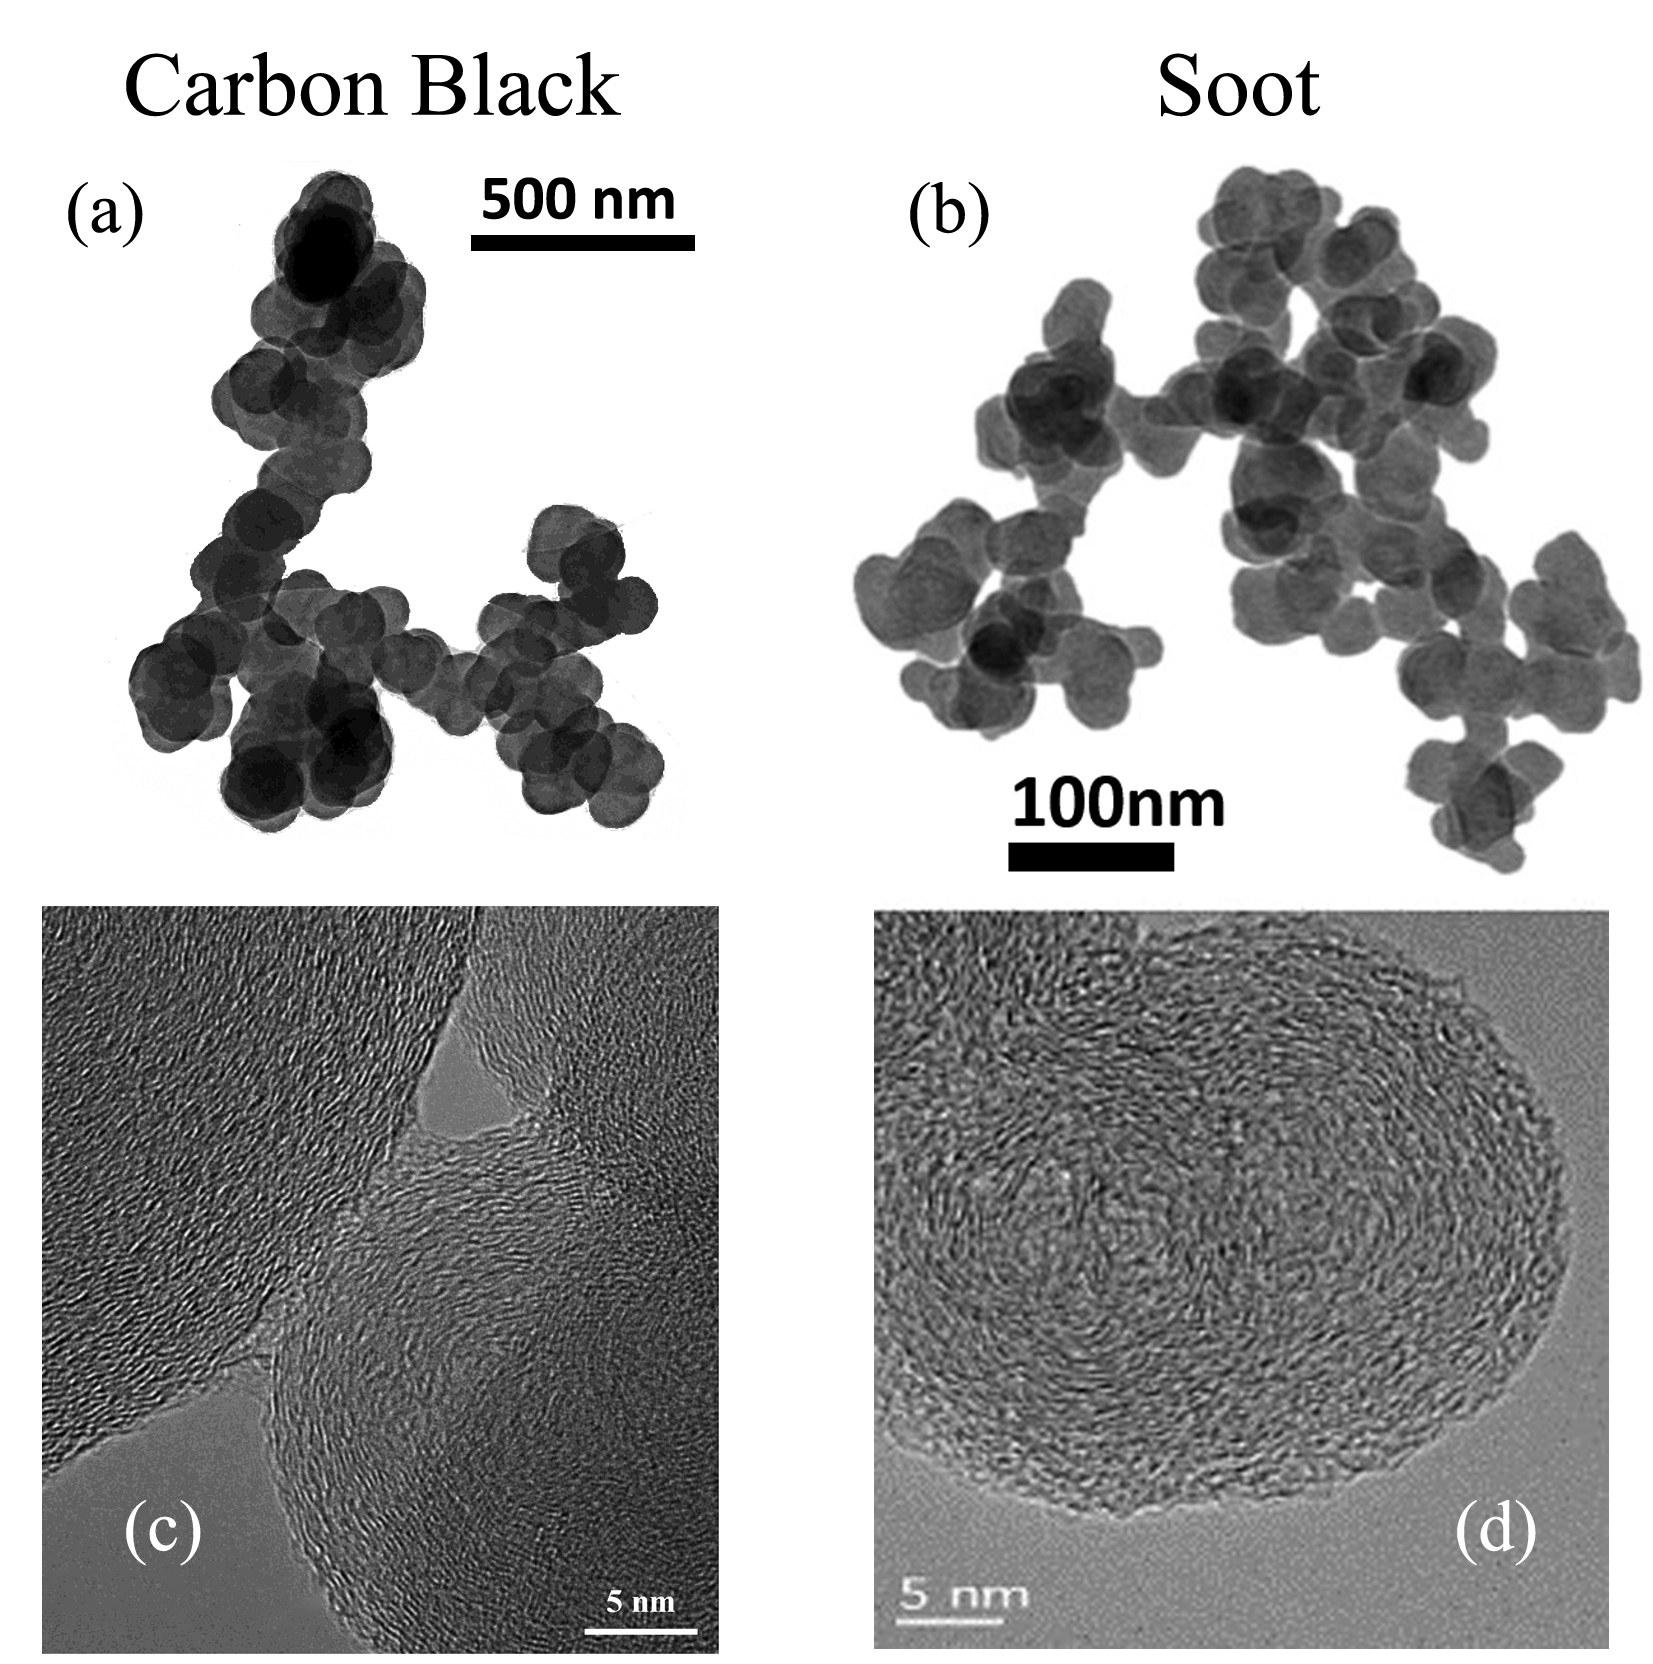
\includegraphics[height=60mm, ]{Figures/Introduction/soot_CB_HRTEM.jpg}
	\caption{The TEM images of Carbon black (a \& c)~\citep{singh2018nanostructure} and soot (b \& d)~\citep{vander2007hrtem, lapuerta2017morphological}
	\label{fig:sootCBHRTEM} that shows soot and CB has similar morphology and structure}
\end{figure} 



\section{Background}
\subsection{Soot inception and surface growth}
The physics of soot formation involves concurrent processes with different time and length scales starting from the breakdown of hydrocarbon molecules to intermediate species and radicals that transition to first soot particles and grow via heterogeneous reactions on the surface as well as coagulation~\citep{d2009combustion}. The TEM analysis of soot sampled from flames~\citep{lapuerta2017morphological}, reactors~\citep{ono2017experimental}, and engines~\citep{wei2020morphology} with different fuels and process conditions revealed a common fractal-like morphology characterized as agglomerates of spheroidal primary particles. High resolution transmission electron microscopy (HRTEM) revealed cluster of precondensed Polycyclic Aromatic Hydrocarbons (PAHs), such as benzene, naphthalene and pyrene, in organized graphitic shell and disoriented core laryers cluster soot primary particles~\cite{alfe2009structure}. Moreover, PAHs can resist dissociation under high flame temperatures due to the thermodynamic stability~\cite{stein1985high} supporting the widely accepted hypothesis that PAH are the main soot precursors. 

However, the transition PAHs (soot precursors) to incipient soot, known \textit{soot inception} has not been well understood at the level of pathways and elementary reactions~\cite{Wang2011} primarily due to uncertainties in PAH (precursor) chemistry. The thermodynamics of PAH growth from acetylene ($\mathrm{C_2H_2}$) as the dominant hydrocarbon species in fuel pyrolysis and an
intermediate of molecular growth does not experience a significant enthalpy release or entropy increase, so the path is driven by a gradual reduction in Gibbs free energy. As a result, the kinetics of PAH growth into 
subsequent soot particles can be highly reversible hence sensitive to local temperature, pressure and intermediate species concentration.

The growth of PAHs beyond first ring (benzene) is predominantly driven by so-called hydrogen abstraction carbon (acetylene) addition (HACA) mechanism~\citep{frenklach2002reaction} where a hydrogen radical abstracts an hydrogen atom at the edge of PAH, providing a reactive site for acetylene addition. The kinetic reversibility of HACA opens the door for competing pathways such as chain reactions of resonance-stabilized radical (RSR). Propargyl is a prominent example of these radicals, whose combination is known as a major contributor to benzene formation~\citep{fahr1989reactions}. Built on this hypothesis, \citet{johansson2018resonance} proposed a radical-driven growth mechanism by addition of vinyl ($\mathrm{C_2H_3}$) starting from cyclopentadienyl ($\mathrm{C_5H_5}$) to larger hydrocarbon radicals that can survive long enough in high temperatures to react with other radicals, PAHs and unsaturated aliphatic species,
through radical chain reactions. However, low concentrations of these radicals limit the growth rate through RSR pathways~\citep{frenklach2020mechanism}. Moreover, some of the intermediate steps for radical regeneration such as formation of vinylcyclopentadienyl were shown to be kinetically unfavorable~\citep{frenklach2020mechanism} compared to HACA. Regardless of their mechanistics, these sequential growth mechanisms, termed as \textit{chemical growth} cannot account for rapid soot formation~\citep{frenklach2002reaction} and its nanostructure~\citep{frenklach1988comment}.

There is abundant but mostly indirect experimental and computational evidence pointing to a collision-based mechanism for soot inception. HRTEM images of
nascent and mature soot shows a disordered PAH clusters highlighting the role of PAH collisions. 
%It was suggested the chemical and collisional growth act as complementary pathways~\citep{d2009nanoparticles}, and their relative strength depend on temperature and fuel composition~\citep{frenklach2002reaction}.  
The bimodality of particle size distribution (PSD) of nascent soot particles in premixed flames~\citep{zhao2003measurement} indicates that the kinetics of inception is second order in precursor concentration~\citep{abid2009quantitative}. The time-of-flight mass spectrometry (TOFMS) experiments in a 13 kPa acetylene-oxygen flame showed a series of peaks with a
periodicity of 500 amu~\citep{happold2009soot}. However, it is not how PAH clusters form and what force allows the binding occur and resist dissociation at the flames temperature ($\ge$ 1600 T). \citet{frenklach2002reaction} characterized the clustering as a physical process where the sticking of PAHs upon collision forms dimer held together by Van der Waals forces without involving chemical reactions. In fact, \citet{herdman2008intermolecular} found that the binding energy of PAHs dimers due to dispersive and electorstatic forces increases linearly with molecular mass and reaches the limit of exfoliation energy for graphite. However, the entropy barrier of dimerization increases with PAH size making them unfavorable under equilibrium conditions. So, PAHs as large as circumcoronene ($\mathrm{C_{54}H_{18}}$) can only form dimer to survive flame temperatures~\citep{Wang2011}. However, the concentration of large PAHs are too low to account for the observed number density of soot particles in flames~\citep{totton2012quantitative}. PAH clustering can also be governed by non-equilibrium kinetics. PAH molecules can for rovibrationally excited dimer with long enough life time~\cite{wong2009molecular} to react with H atoms forming covalent bonds. There is also possibility for these clusters to joined by aliphatic linkages. Micro-FT-IR spectroscopy analysis by \citet{cain2011evidence} showed the ratio of aliphatic-to-aromatic C–H bonds can exceed unity at flame temperature. Using these findings, they suggested that
the aliphatic components in the form of alkyl,
alkenyl can covalently bound to aromatic units in soot particles. Although such a mechanism is viable near the flame region, it cannot explain persistent soot inception in the post flame zone~\citep{zhao2005particle} where the H atom concentration is too low to initiate H abstraction reactions that produce those radicals.

\begin{figure}[!htbp]
	\centering
	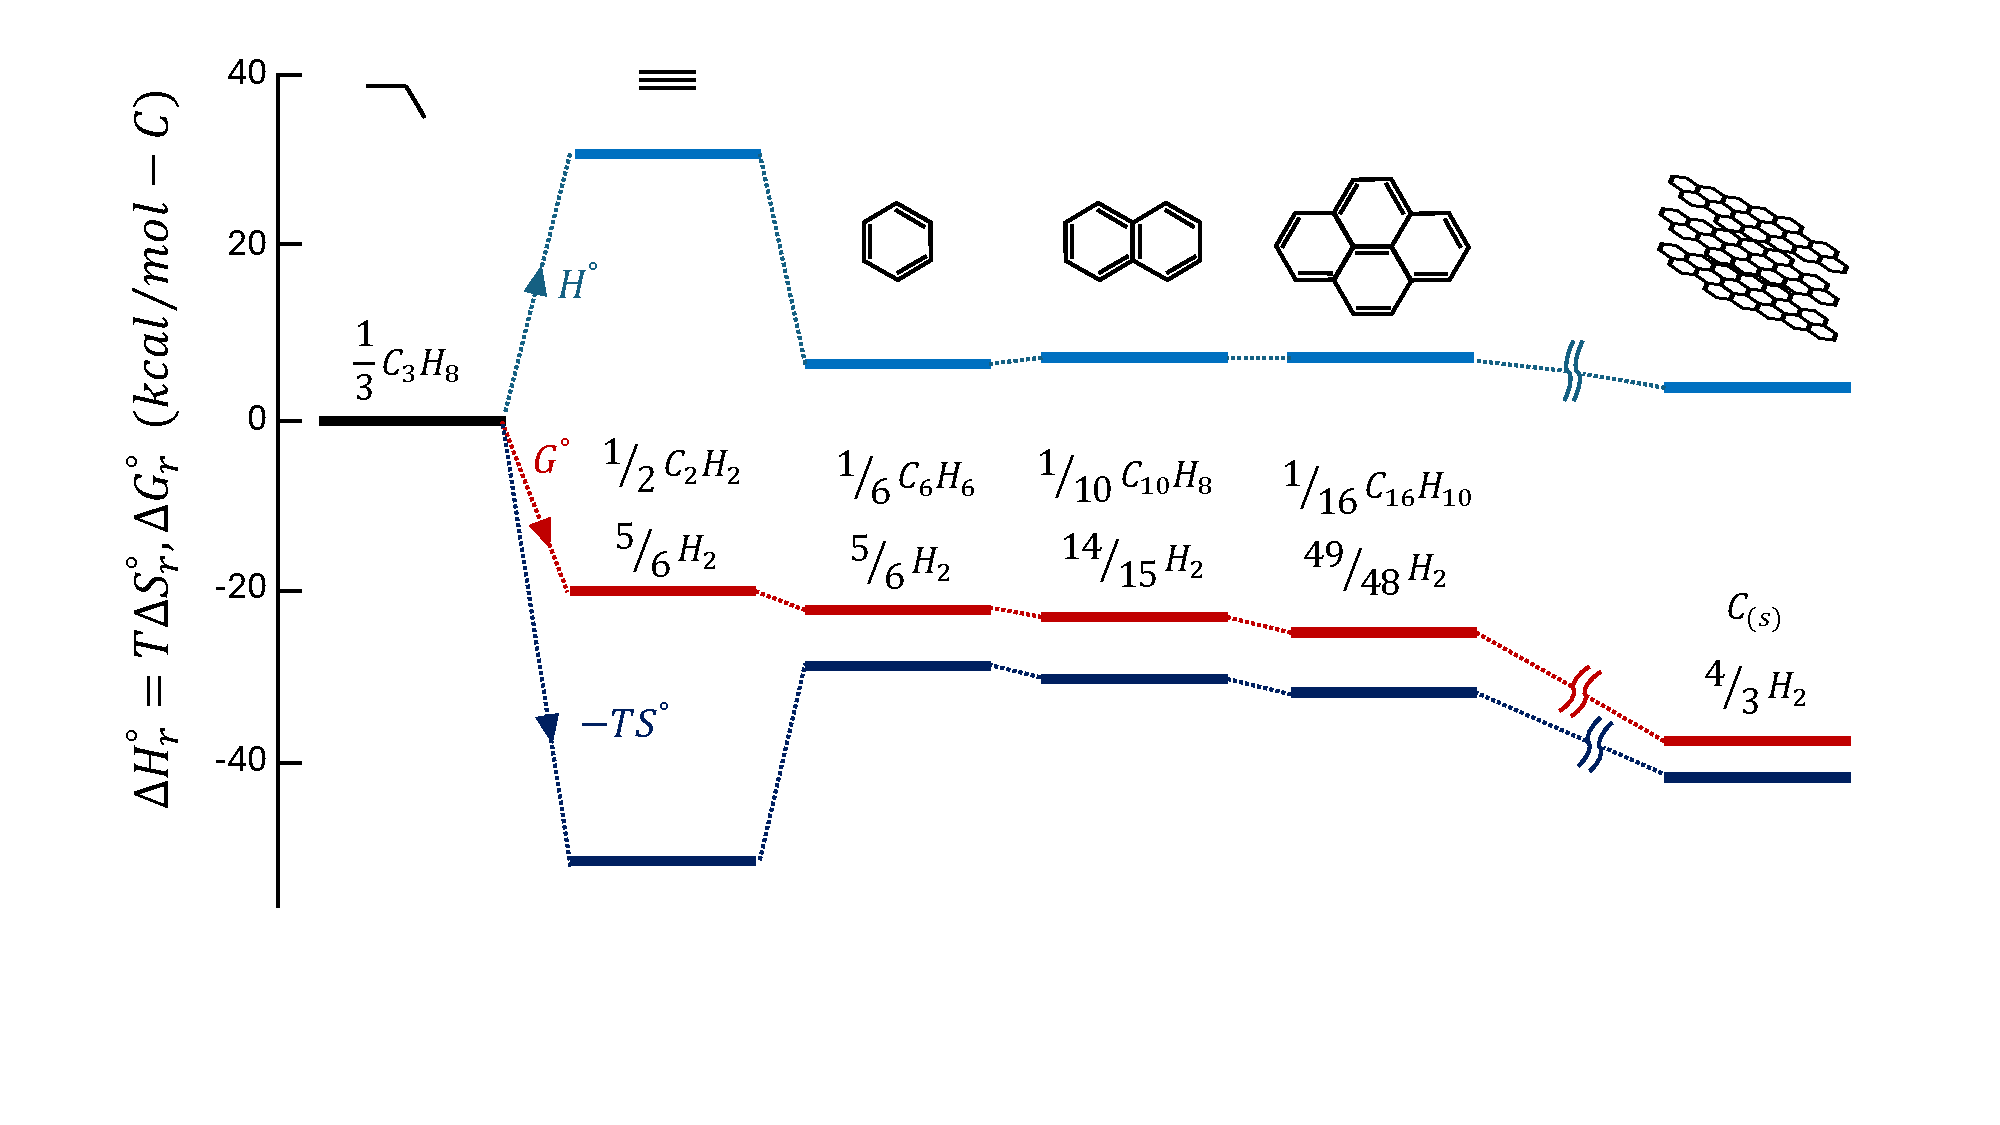
\includegraphics[height=60mm, ]{Figures/Introduction/gibbs_propane.pdf}
	\caption{Standard enthalpy (${\Delta H}$) and entropy (${T\Delta S}$) contributions to Gibbs function of reaction $\mathrm{\Delta F}$ at 1600 K for carbon formation from propane(reprinted from ref.~\citep{Wang2011})}
\end{figure} 

There are other complicating factors that hinders the fundamental understanding of soot inception such as lack of a decisive criterion to distinguish gaseous molecules from particles~\citep{d2009combustion}, and the overlap of inception with surface growth and agglomeration~\cite{martin2022soot}. Measurement techniques have limited capability in soot detection due to short time and length scales of soot inception and surface growth ranging from pico- to milliseconds and micro- to millimeter~\citep{violi2005relative}. Fig.\ref{fig:sootscales} demonstrates the length and time scales relevant to different stages of soot formation from PAH precursors to incipient, nascent and mature soot in flames. Moreover, the collected data from measurements might not be the true representative of soot formed at the probed location of the studied process. For example, intrusive diagnostic methods based on thermophoresis or dilution have a sampling probe that can perturb flow dynamics or alter structure and composition of soot~\cite{kholghy2017comparison}. Non-intrusive techniques such as optical methods also rely on assumptions about light absorption and scattering of soot~\citep{shaddix1996laser} and its morphology~\citep{doner2017impact}.
Despite the gaps in fundamental understanding of soot formation and limitations of diagnostics methods, models have been developed describe the soot inception and growth. These models have been formulated as a set of clear pathways that explain soot inception based on collisions of PAH molecules. They have to be consistent with current knowledge of soot physics, feasible to be coupled with chemistry and particle dynamics models, and able to predict soot mass, PSD and morphology observed in flames and reactors.

Soot inception was originally described as PAH dimerization where collision of two PAH molecules (monomers in this context) forms a dimer held together by Van der Wales forces~\citep{frenklach1991detailed}. The dimerization is a irreversible process with a efficiency that accounts for the reversibility or dissociation of dimers. The theory postulates that PAH growth continues by sequential addition of a monomer (PAH molecule) forming stacks of dimers, trimers, tetramers and so on to reach a certain mass threshold that marks the emergence of incipient soot~\citep{frenklach1991detailed}, but for practical purposes, a dimer is usually considered as incipient soot. Here, we call this model \textit{Irreversible Dimerization}. 
Irreversible Dimerization has been used to predict soot formation in burner-stabilized premixed~\citep{salenbauch2015modeling, desgroux2017comparative}, counterflow diffusion flames~\citep{wang2015soot, xu2021experimental}, coflow diffusion flames~\citep{kholghy2016core, veshkini2016understanding}. A collision efficiency factor ranging between $10^{-6}$ to 1 is also employed to adjust the inception flux and PAH adsorption rates to achieve desired soot mass and size distribution. PAHs of moderate sizes such as pyrene (4 rings) to coronene (7 rings) have been considered as the starting point of inception due to their thermodynamic instability that justifies the irreversibility at high temperatures~\citep{frenklach1991detailed}. \citet{blanquart2009analyzing} introduced a two-step However, the theoretical calculations~\citep{miller1985calculations} and experiments~\citep{sabbah2010exploring} indicated that pyrene dimerization is highly reversible in flame condition.



% Fringe analysis from Jacob's paper 

%  “chemical similarity” hypothesis in "Unified Kinetic Model of Soot Formation in the Pyrolysis and Oxidation of Aliphatic and Aromatic Hydrocarbons in Shock Waves"

% Maybe use discussion in nucleation flame paper to argue for a collision-based proxy inception model 

%  are limited by possible ~\citep{buesser2012design} due to coupling with gas chemistry~\cite{Wang2011}, dependence on local temperature~\citep{gleason2018effect} and pressure~\cite{gleason2021pahs}. It has also been challenging to pinpoint the start of inception because of its short time scales in the order $10^{-9}$ s~\citep{buesser2012design}, the lack of a decisive criterion to distinguish molecules from particles~\citep{d2009combustion}, and the overlap of inception with particle growth and agglomeration~\cite{martin2022soot}. Despite these limitations and challenges, our knowledge about soot formation has significantly increased thanks to advances in diagnostics methods and reaction mechanism development. 

\begin{figure}[!htbp]
	\centering
	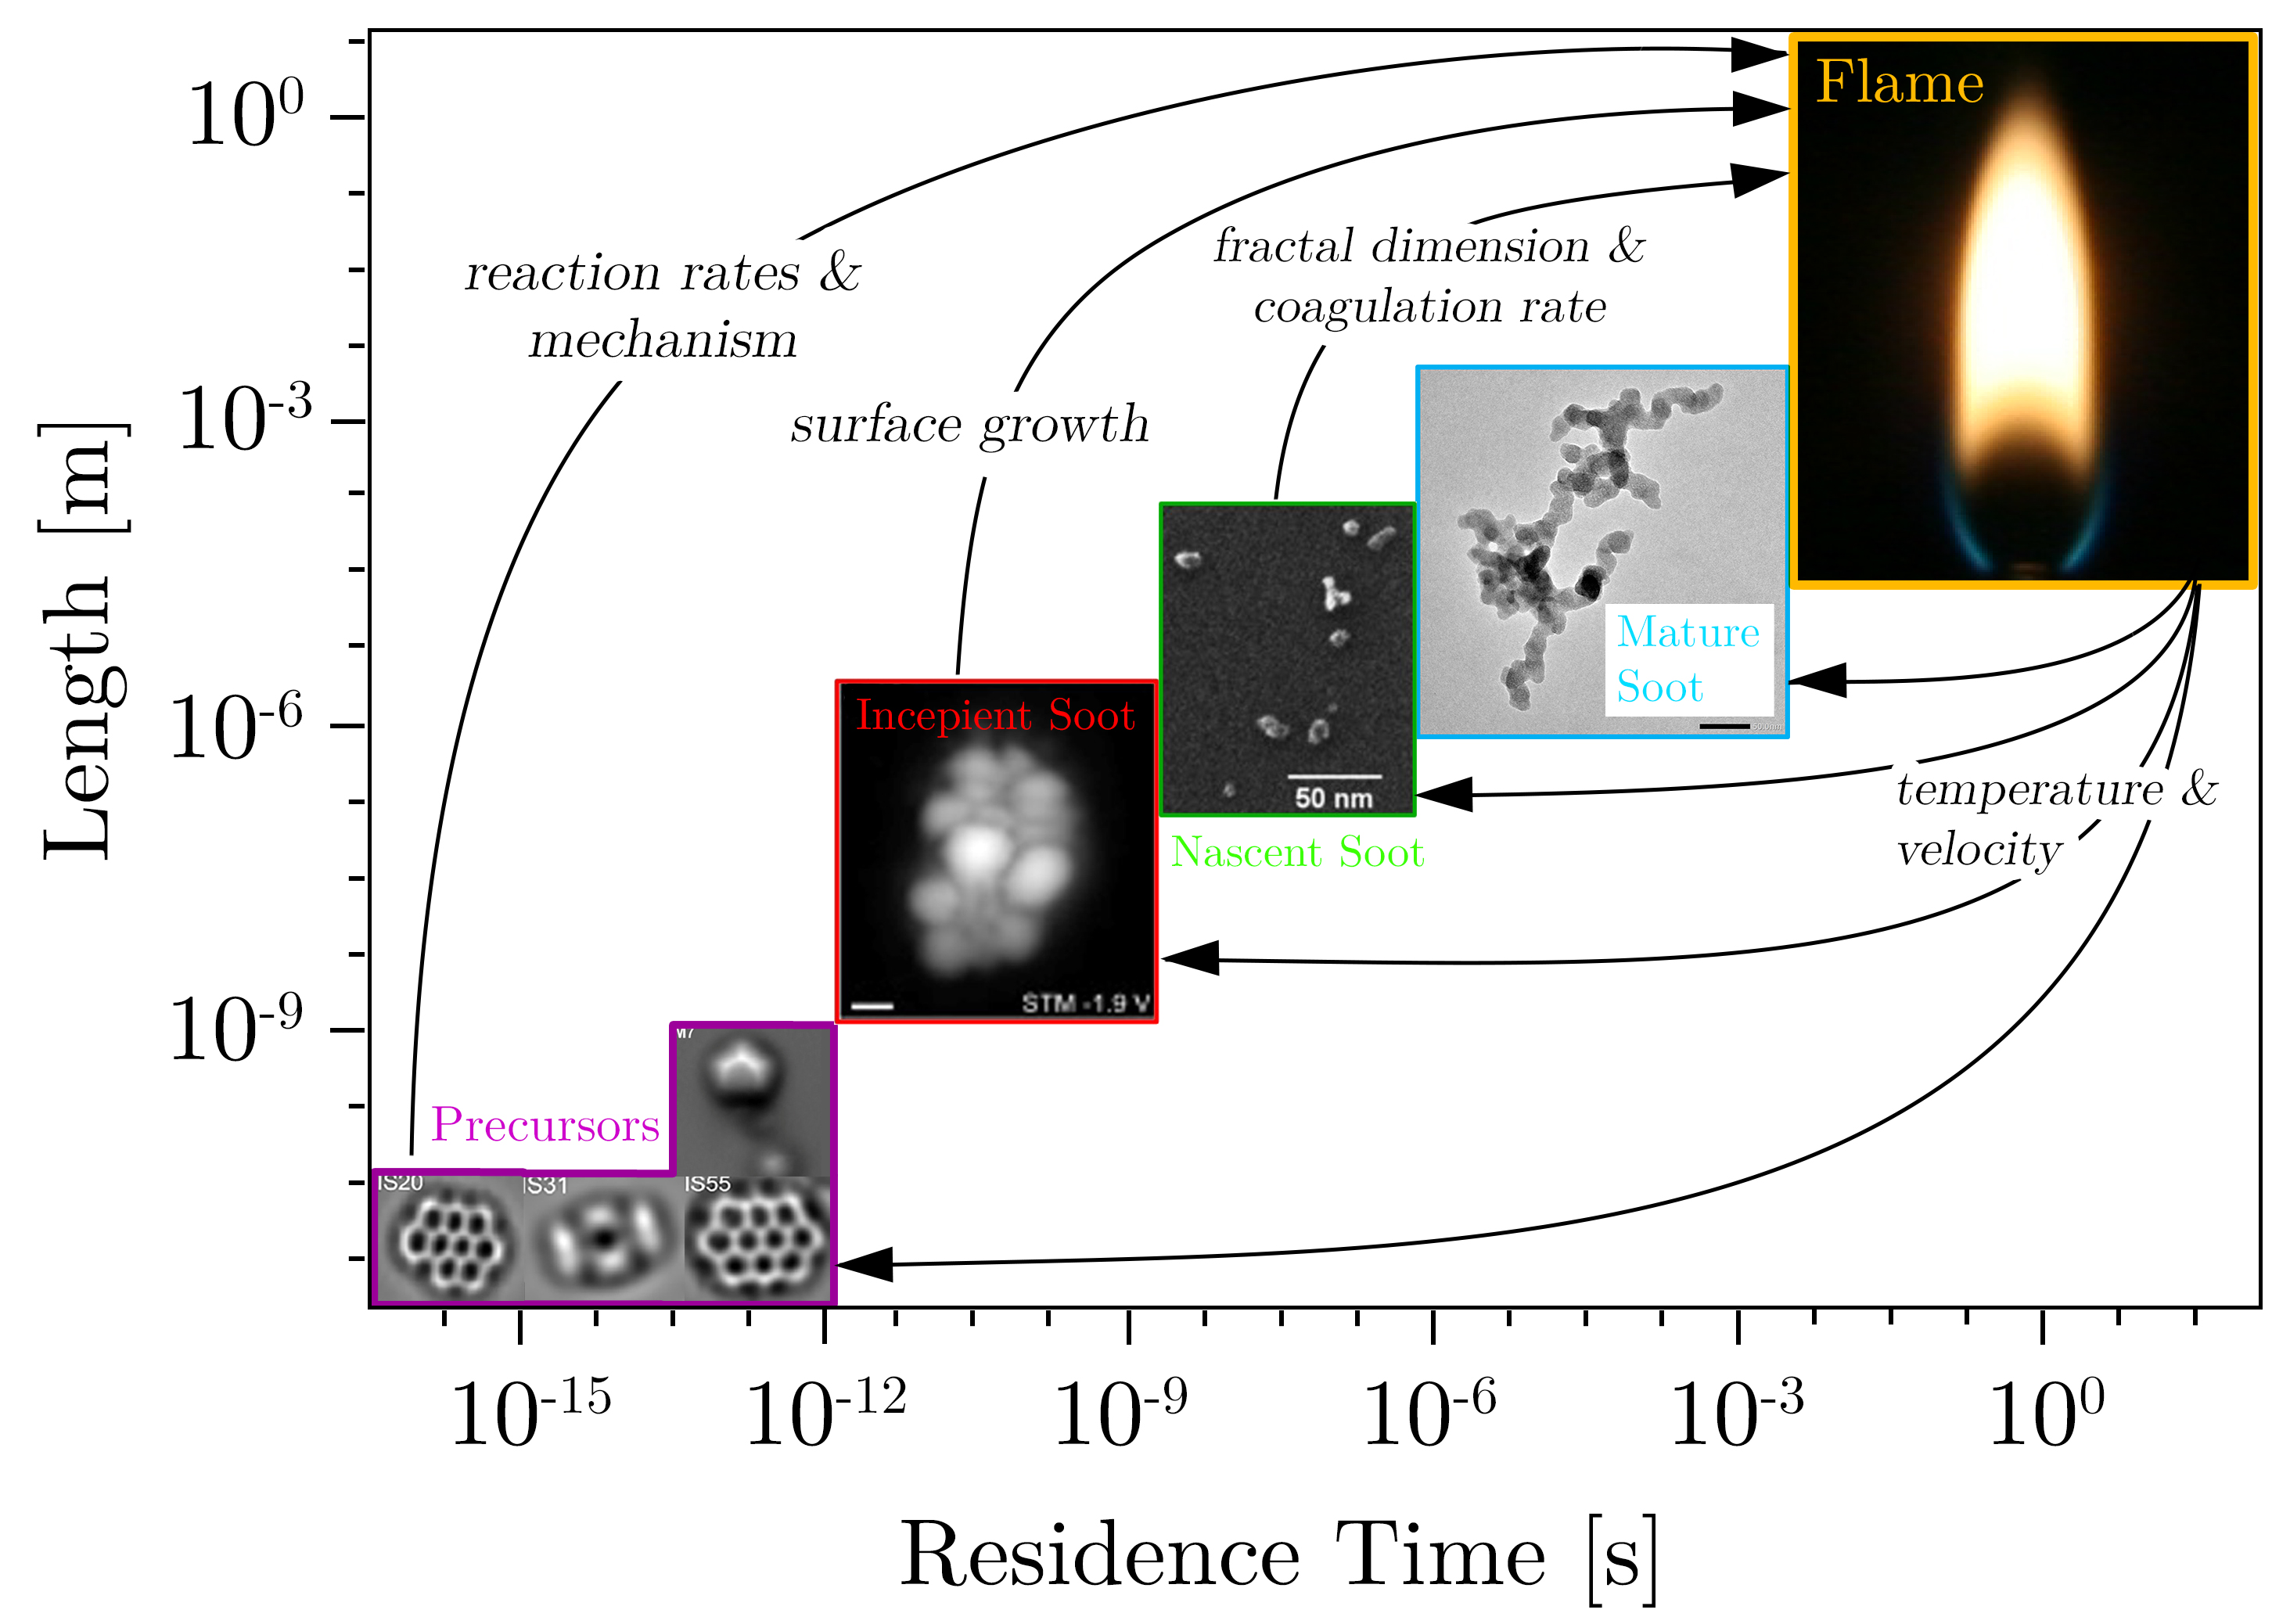
\includegraphics[height=80mm, ]{Figures/Introduction/schematics.jpg}
	\caption{The range of time and length scales of the processes involved in soot formation from molecular reactions to particle-fluid interaction in flames}
	\label{fig:sootscales}
\end{figure}



%There is compelling evidence that highlights the role of Polycyclic Aromatic Hydrocarbons (PAH) as the main soot precursors. They are thermodynamically stable enough to withstand dissociation at high flame temperatures~\citep{stein1985high} and observed in stacked layers in High Resolution Transmission Electron Microscope (HRTEM) images of soot primary particles~\citep{Oberlin1984}. 
%\hl{[placeholder for literature review on the role of diradicals and resonantly stabilized radicals in soot inception]}

%But, the two important questions need to be answered: (1) which PAHs contribute most to the inception, and (2) what pathways best describe PAH to incipient soot transition. Purely chemical growth mechanisms are shown to underpredict inception rates and particle size~\citep{frenklach2002reaction}. The bimodality of particle size distribution in premixed flames~\citep{camacho2015mobility} suggests a mechanism second order with respect to the monomer~\citep{Wang2011}. To satisfy these requirements, a collision-based inception was proposed where irreversible polymerization form PAH clusters held together by Van der Wales forces. The theory postulates that PAH growth continues to reach a certain mass threshold that marks emergence of solid particles, but for practical purposes, a dimer is usually considered as incipient soot. 

%In this model, hereafter referred to as \textbf{Irreversible Dimerization}, the collision of two PAH molecules is assumed to form a dimer
% that gains mass via two growth mechanisms: (i) hydrogen-abstraction-carbon-addition (HACA) that assumes soot surface to consist of hydrogenated sites with predefined density that can lose hydrogen and react with acetylene (ii) collision of PAH molecules/clusters with soot particles leading to chemisorption. 
 

The inception rate of irreversible dimerization is mainly controlled by PAH concentration due to weak temperature dependence, so it produces new particles in low temperatures (even less than 500 K)~\citep{naseri2022simulating} despite experimental evidence for termination of inception below 1200 K~\citep{sanchez2012polycyclic, cho2016synthesis}. Also, the arbitrary selection of efficiency factors alters the distribution of mass between inception of surface growth the could significantly change soot mass, PSD, and morphology strongly~\citep{saffaripour2014experimental}. \citet{miller1991kinetics} used equilibrium constant for PAH dimerization to calculate the net dimerization rate and demonstrated that the collision of PAHs larger than circumovalene ($\sim$800 amu) could last long enough grow into incipient soot. However, the concentration of PAHs drops rapidly with size~\citep{Wang2011}. The entropy barrier of dimerization is significant for larger PAHs~\citep{giordana2011theoretical}.  


\citet{eaves2015importance} relaxed the irreversibility assumption, and developed a reversible clustering model to simulate inception using an array of PAHs from naphthalene to benzo-pyrene. Building on that work, \citet{kholghy2019role} emphasized on the necessity of chemical bond formation after physical PAH clustering for accurate prediction of volume fraction, primary particle diameter and PSD in ethylene coflow diffusion flames. Later, \citet{kholghy2018reactive} proposed the \textit{"Reactive Dimerization"} model which starts with reversible collision of PAHs leading to physical dimers held with vdW forces that are graphitized and form chemically-bonded dimer that serve as soot nuclei grow via surface reactions. They also performed a systematic analysis on contribution of different PAHs, and concluded that one- and two-ring aromatics account for almost all of inception flux in the so-called \textit{"sooting flame"}~\citep{desgroux2017comparative}. However, \citet{frenklach2020mechanism} pointed out that an inception model that initiated with a highly reversible step similar to Reactive Dimerization~\citep{kholghy2018reactive} cannot produce sufficient flux of particles to match measurements of the benchmark burner-stabilized stagnation flame~\citep{abid2009quantitative}. Instead, they proposed a HACA-driven mechanism where addition of monomer molecule to its radical activated by hydrogen abstraction for a stable dimer via an E-Bridge bond formation, and this sequential process continues to form trimers, tetramers, and larger PAH clusters.

The gas-phase chemistry of aromatics can be extended to account for chemical growth of incipient soot via surface reactions~\citep{frenklach2002reaction}. This hypothesis, known as “chemical similarity” postulates that the reactions occurring on the soot surface are similar to those involving large molecules of PAHs in the gas phase. It also provides means to describe the rates of surface growth and particle oxidation in
terms of elementary chemical reactions. In other words, it is assumed that the surface of soot particles is made up of lateral faces of larges PAHs covered with C-H bonds.
This is the basis for the hydrogen–abstraction–acetylene–addition (HACA) mechanism~\citep{frenklach1991detailed, appel2000kinetic}  that assumes the soot surface to consist of hydrogenated sites with a predefined density. Mass growth on soot surface requires H-abstraction to form a radical
site, followed by acetylene attack similar to growth of PAH molecules in the gas-phase. The reactivity of these sites changes with time and temperature~\citep{woods1991soot, dasch1985decay}, described as soot aging. Fr modelling purposes, a temperature-dependent multiplier, usually represented by $\alpha$, was introduced to account for these effect. \citet{appel2000kinetic} showed $\alpha$ changes with temperature and particle size. However, soot mass growth without the presence of H radicals~\citep{singh2006numerical} indicated the incompleteness of the HACA mechanism to
describe the entire process of soot surface growth.

Adsorption of PAHs on the surface of soot particles is also a viable growth mechanism~\citep{frenklach1991detailed}, more specifically called physiorption or chemisorption depending on the mechanisms driving the adsorption process~\citep{michelsen2020review}. There is still debate over the stability of adsorbed PAH molecules on soot surface~\citep{obolensky2007interplay}. Following the hypothesis that PAHs are building blocks of soot particles, a mechanism similar to inception is often used to describe  PAH-soot growth.

\section{Coagulation and agglomeration}

In typical soot formation processes such as flames and reactor, soot particles are formed at high concentrations ($\mathrm{10^{12}}$ $\mathrm{1/cm^3}$), and inception and surface growth are relatively short compared to the total residence of soot particles. As a result, coagulation becomes dominant rapidly attaining both~\citep{Goudeli2016}
self-preserving size distribution (SPSD)~\citep{lai1972self} and asymptotic fractal-like structure~\citep{mountain1986simulation}.
The evolving fractal-like structure of agglomerates quantified by their mobility diameter normalized by primary particle, $d_m$⁄$d_p$, and gyration, $d_m$⁄$d_g$, diameters can be described with power laws derived from mesoscale simulations~\citep{Kelesidis2017}. The collision frequency of agglomerates depends on their evolving fractal-like morphology. Also, polydisperse agglomerates collide more frequently than monodisperse ones. The enhancement in their collision frequency reaches an asymptotic value of 35\%~\citep{Goudeli2016} or 82\%~\citep{kelesidis2021self} in the free molecular or transition regimes, respectively at SPSD regardless of the polydispersity in their constituent primary particles. Particle morphology formed by inception, surface growth and agglomeration can be tracked precisely by mesoscale simulations, such as Discrete Element Modeling (DEM)~\citep{Kelesidis2017Flame}. However, they are computationally expensive and interfacing them with chemical kinetics in computational fluid dynamics (CFD) simulations is not trivial~\citep{kelesidis2021perspective}. This limits their application. So, sectional population balance models (SPBM) are often used to track agglomerate and primary particle size distribution~\citep{Xiong1993}, morphology~\citep{park2005aerosol}, and composition~\citep{kholghy2016core} in complex laminar~\citep{kholghy2016core} and turbulent flows~\citep{schiener2019transported}. Using the SPBMs coupled with relations for agglomerate fractal-like structure~\citep{matsoukas1991dynamics} and collision frequency [36], particle size distribution, morphology and composition can be tracked accurately. However, the computational cost of SPBMs increases exponentially with the number of sections [31] and particle properties~\citep{kholghy2016core} tracked. Thus, one property (e.g. agglomerate mass) is typically tracked with SPBMs to reduce computational cost. This does not allow to account for agglomerate fractal-like structure~\citep{smooke2005soot, aubagnac2018soot} which limits SPBM accuracy in predicting surface growth and coagulation rate of agglomerates and their size distribution.

Alternatively, particle dynamics can be tracked by the method of moments (MOM)~\citep{kazakov1998dynamic} or monodisperse population balance models (MPBM)~\citep{kruis1993simple}. Such models only track average particle properties (e.g. moment ratios) and their accuracy could be limited if unrealistic assumptions (e.g. approximating agglomerates as monodisperse and perfect spheres) are used. However, when inception and surface growth are short~\citep{Spicer2002} and high particle (number) concentrations are formed~\cite{Kelesidis2017}, they lead to rapid attainment of self-preserving size distributions (SPSD) and agglomerates having asymptotic structure~\citep{Goudeli2016}. In this case a MPBM or MOM can be assembled on a firm scientific basis with accuracy on par with DEM~\citep{Kelesidis2017Flame}, SPBM~\citep{kelesidis2019estimating} and experimental data ~\citep{abid2008evolution, ma2013soot, camacho2015mobility}. Such models can be readily interfaced with CFD simulations~\citep{grohn2012fluid} without significant computational cost, making them ideal for three-dimensional and even turbulent flame simulations. 

The MOM tracks moments of the PSD and estimates average particle properties such as mass~\citep{pratsinis1988simultaneous}, surface area~\citep{blanquart2009joint}, the number of constituent primary particles per agglomerate, $\mathrm{n_p}$~\citep{kazakov1998dynamic}, or even particle compositio~\citep{blanquart2009analyzing} using the ratio of the moments. The MOM with four equations was used to describe synthesis of optical fibers by simultaneous reaction, diffusion, coagulation and thermophoresis of $\mathrm{SiO_2}$ in laminar flow reactors assuming a lognormal PSD~\citep{kim1988manufacture}. The MOM with interpolative closure (MOMIC) was developed to predict simultaneous nucleation, surface growth and coagulation of soot agglomerates and estimate its PSD with six equations~\citep{kazakov1998dynamic}. To calculate source terms of the transported moments, additional moments that are not tracked are needed preventing the closure of the system of differential equations with the MOM~\citep{pratsinis1988simultaneous, frenklach1987aerosol}. Thus, often the PSD shape is assumed a priori~\citep{pratsinis1988simultaneous} or extra equations are solved to estimate it~\citep{kruis1993simple}.

The MPBMs do not have the closure problem and calculate average particle properties by tracking their total concentration, mass \citep{kruis1993simple} and area~\citep{tsantilis2004soft, lindstedt1994simplified}. \citet{kruis1993simple} used a 2-equation MPBM (known as the semi-empirical model) to track soot concentration and mass in (non-premixed) flames assuming spherical particles. Good agreement was achieved for measured soot mass. However, the specific surface area~\citep{lindstedt1994simplified} and coagulation frequency of spheres are significantly smaller compared to that of agglomerates with the same mass underestimating their oxidation rate~\citep{kelesidis2019estimating} and overestimating their concentration [40]. \citet{kruis1993simple} proposed a 3-equation MPBM to account for the fractal-like structure of nanoparticle agglomerates during coagulation and sintering. Agglomerate volume and area were used to obtain their equivalent primary particle diameter, $\mathrm{d_p}$, and $\mathrm{n_p}$. Then, agglomerate collision diameter, i.e. $\mathrm{d_g}$, was calculated by $\mathrm{D_f}$, $\mathrm{d_p}$ and $\mathrm{n_p}$ to account for their fractal-like structure that affects their collision frequency. \citet{tsantilis2004soft} extended the MPBM to predict hard-(chemically-bonded) and soft- (physically-bonded) agglomerates during synthesis of $\mathrm{SiO_2}$ and $\mathrm{TiO_2}$~\citep{grass2006design} nanoparticles with simultaneous reaction, surface growth, coagulation and sintering. Such a MPBM applies best at high concentrations when inception and surface growth are short~\citep{Spicer2002} resulting in the dominance of coagulation where particles rapidly reach their SPSD and asymptotic fractal-like structure. This is often the case for soot emitted from a variety of combustion devices or CB reactors where inception and surface growth are limited to only a few milliseconds when temperature is very high (i.e. T$\ge$1500K)~\citep{kholghy2018reactive}.

\section{Soot maturity and its optical properties}
The maturity level of soot is described as the evolution of physical and chemical properties from incipient to graphite-like mature soot~\citep{michelsen2017probing}. It involves the growth of the graphitic crystallite fine structure of soot within,
and perpendicular to, the aromatic layers.~\citep{franklin1951crystallite, haynes1981soot}, known as graphitization, followed by increase in the size of
the crystallite-layer planes and decrease of the interlayer spacing~\citep{alfe2009structure}. This process is accompanied by the pyrolytic conversion of hydrocarbon species and substituted hydrocarbons toward elemental carbon and increase in the carbon-to-hydrogen (C/H) ratio, known as carbonization. Soot maturity is closely associated with reactivity of surface sites. At early stages of formation, soot surface is considerably more reactive than that of mature graphitized mature soot~\citep{camacho2015kinetics}. Fig.\ref{fig:sootmaturity} compares nanostructure of nascent soot composed of disoriented PAH clusters with that of mature soot with a core-shell pattern where disordered core is surrounded by concentrically oriented graphitic layers~\citep{happold2009soot}. The core-shell nanostructure of mature soot strongly depends on process conditions such as pressure, fuel identity, temperature and residence time of the particles. 

Evolution of soot maturity and morphology impacts its optical properties. Incipient and nascent soot absorb shorter wave lengths ($\lambda$<600 $\mu m$) as opposed to mature soot particles that are broad-band light absorbers~\citep{hurt2000equilibrium}. Non-intrusive optical diagnostic methods such as light extinction (absorption and scattering)~\citep{mcenally1997soot} and Laser Induced Incandescence (LII)~\citep{shaddix1996laser} are widely utilized to measure soot volume fraction, $f_v$ using extinction coefficient and the absorption function, E(m) that depends on soot refractive index, m, soot composition and morphology~\citep{desgroux2013study}.

\begin{figure}[!htbp]
	\centering
	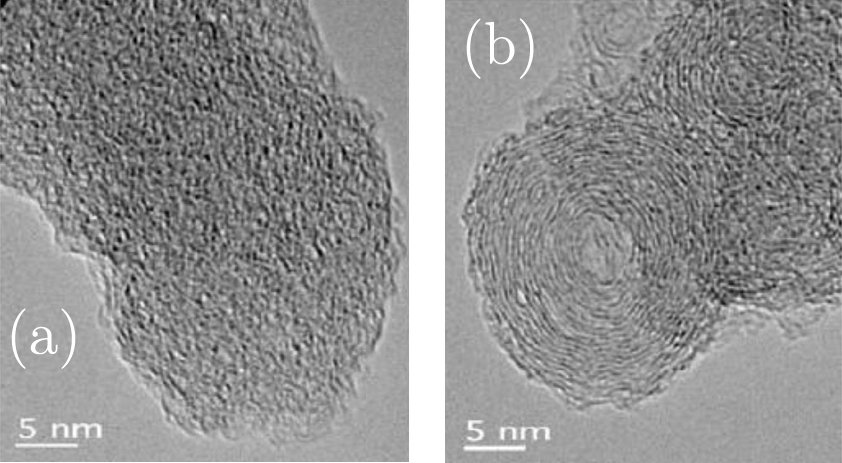
\includegraphics[height=40mm, ]{Figures/Introduction/soot_maturity.jpg}
	\caption{The HRTEM image of (a) a nascent soot primary particle with disordered internal nanostructure juxtaposed with that of (b) a mature soot primary particle with well-organized cluster near the shell sampled from soot generated by pyrolysis of ethanol at 1250 and 1650, respectively. Reprinted from Ref.\citep{vander2004soot}}
	\label{fig:sootmaturity}
\end{figure}


However, the effects of soot composition, and morphology on its m, and E(m) are not fully understood yet. E(m) of soot at $\lambda=$1064 nm measured by two-color LII measurements increases from 0.193 to 0.349, and 0.226 to 0.340 for ethylene premixed flames with equivalence ratio of $\phi$=2.1 and $\phi$=2.3, respectively when height above burner (HAB) changes from 8 to 14 mm~\citep{olofsson2015evolution}. During acetylene pyrolysis in a shock tube, E(m) of soot particles increases from 0.05 to 0.25 as their primary particle diameter, $d_p$, grows to 20 nm within 1.6 ms~\citep{eremin2011size}. Using m and E(m) of mature spherical soot~\citep{dalzell1969optical} at different HABs neglecting the impact of soot morphology and composition on m~\citep{zerbs2009influence} can overestimate soot volume fraction by 100\%~\citep{kelesidis2021determination}. So, accurate estimation of the evolving optical properties of soot is essential to close the carbon mass balance in the measurements~\citep{kelesidis2021determination}, and analyze reaction kinetics for soot inception~\citep{kholghy2018reactive} surface growth~\citep{appel2000kinetic} and oxidation~\citep{puduppakkam2014soot} that are essential for development and validation of aerosol dynamics models coupled with chemistry to predict soot formation.


The dependence of soot m on its morphology and composition can be quantified by soot optical band gap, $\mathrm{E_g}$~\citep{bond2006light}. The optical band gap concept was originally proposed by \citet{tauc1966optical} for semi-conductors and later developed for amorphous carbon~\citep{robertson1987electronic}, and it can be used to describe the crystalline character of PAH clusters in soot~\citep{robertson1987electronic}. Incipient flame-made soot with diameters less than 20 nm exhibit quantum dot behavior~\citep{liu2019flame} with 0.7$< \mathrm{E_g}<$2 eV that is larger than $\mathrm{E_g}$ of graphitized soot, 0.12 eV~\citep{liu2019flame}. Optical band gap of organic carbon coated on soot remains nearly constant (~1.8-1.9 eV) over soot evolution~\citep{le2019soot}. In contrast, \citet{russo2020optical} measured soot optical band gap using ex-situ and in-situ methods and showed that $\mathrm{E_g}$ drops from 0.7 eV at HAB= 8 mm to 0.2 eV at HAB=14 mm in an ethylene premixed flame with $\phi$=2.3 as particles grow and become more mature by carbonization. \citet{kelesidis2019soot} correlated the evolving m of soot with its $\mathrm{E_g}$ obtained from quantum confinement theory (QCT)~\citep{liu2019flame} for wavelengths of $\lambda$= 532 and 1064 nm~\citep{kelesidis2019soot} by linear interpolations between that of nascent ($\mathrm{E_g}$ = 0.60 eV~\citep{minutolo1996optical}; m = 1.51-0.33i and m = 1.48-0.24i for $\lambda$= 532 and 1064 nm, respectively~\citep{bond2006light, moulin2008optical}) and mature soot ($\mathrm{E_g}$ = 0.25 eV~\citep{minutolo1996optical}; m = 1.66–0.76i and m = 1.78-0.92i for $\lambda$= 532 and 1064 nm, respectively~\citep{yon2015radiative}). The proposed relations were then used with soot morphologies obtained from Discrete Element Modeling (DEM) simulations to obtain the evolving Mass Absorption Cross-section (MAC), E(m), and the absorption function ratio of soot (E($\lambda$=532nm)/ E($\lambda$=1024nm)) and compared with measurements~\citep{bejaoui2015measurements, michelsen2010wavelength, cleon2011laser}. Employing the relation in laser diagnostics to reprocess light extinction measurement data resulted in accurate prediction of $f_v$ in moderate ($\phi$=2.34)~\citep{kelesidis2021determination} and rich ($\phi$>3) ethylene premixed flames~\citep{mei2021formation}, and fv along the centerline of a coflow ethylene diffusion flame~\citep{kelesidis2022santoro} which is necessary to close the carbon mass balance in soot generating processes. 

\section{Oxidation}
Soot oxidation is described as the removal of soot mass by reaction of molecular oxygen ($\mathrm{O_2}$), oxygen radical (O), and hydroxyl radical (OH) from soot surface. Because of its heterogeneous reaction kinetics and mechanisms, oxidation is expected to be sensitive to surface structure and composition. So, oxidation mechanisms depend on soot maturity and temperature-time history. In near stoichiometric and fuel-rich conditions, the contribution of OH radical to soot oxidation is predominant~\citep{neoh1981soot} compared to that of O radicals~\citep{lighty2009soot}. \citet{fenimore1967oxidation} investigated soot oxidation rate for low oxygen
partial pressures and temperatures from 1530 to 1890K, highlighted the importance of OH as a major oxidation agent, and attributed the faster rates
compared to those predicted by \citet{lee1962rate}, to OH oxidation. One approach for describing OH oxidation is by a introducing collision efficiency representing the fraction of collisions of OH with soot particles that resulted in the removal of a carbon atom~\citep{neoh1981soot}. Scanning Mobility Particle Sizer (SMPS) with a two-stage burner also
showed a collision efficiency of 0.13~\citep{bartok1991fossil}.

The empirical relation of Nagle and Strickland-Constable (NSC)~\citep{nagle1962oxidation} originally developed for oxidation of pyrolytic graphite have been widely used to describe soot oxidation by $\mathrm{O_2}$. It describes $\mathrm{O_2}$ oxidation rate based on partial pressure of  $\mathrm{O_2}$ and the fraction of eactive edge sites to less reactive basal planes using the graphite analogy for soot. The dominance of edge sites at typical combustion conditions accounts for the relatively small reactivity of soot and basal planes become reactive at high temperature ($>$2500 K)~\citep{lighty2009soot}. $\mathrm{O_2}$ oxidation kinetics was also described with a power-law kinetics \citet{lee1962rate}, and shown first order in oxygen concentration~\citep{neeft1997kinetics}. Alternatively, soot oxidation can be explained based on chemical similarity using HACA mechanism assuming that active site are attached by $\mathrm{O_2}$ and OH leading to loss ot carbon and release of CO.

A different oxidation regime has been identified for soot at low temperatures (T$<$1000 K) where $\mathrm{O_2}$ diffuses and reacts with bulk soot accounting for most of soot mass consumption~\citep{ma2013soot}.  Internal oxidation compacts the pore network of soot resulting in hollow CB~\citep{kelesidis2022porosity}, diesel~\cite{ishiguro1991microstructural} and biodiesel~\citep{song2006examination} soot particles and increases their SSA up to a factor of four~\cite{ishiguro1991microstructural}. Oxidation can cause fragmentation of soot particles affecting their morphology. The increase in number concentration and the change of soot morphology in lean premixed flames ~\citep{xu1997soot} and in the oxidation region of diffusion flames~\citep{puri1993aerosol} was attributed to fragmentation. Such a change in agglomerate morphology has not been observed in fuel-rich conditions, so fragmentation was linked to $\mathrm{O_2}$ oxidation.



\begin{figure}[!htbp]
	\centering
	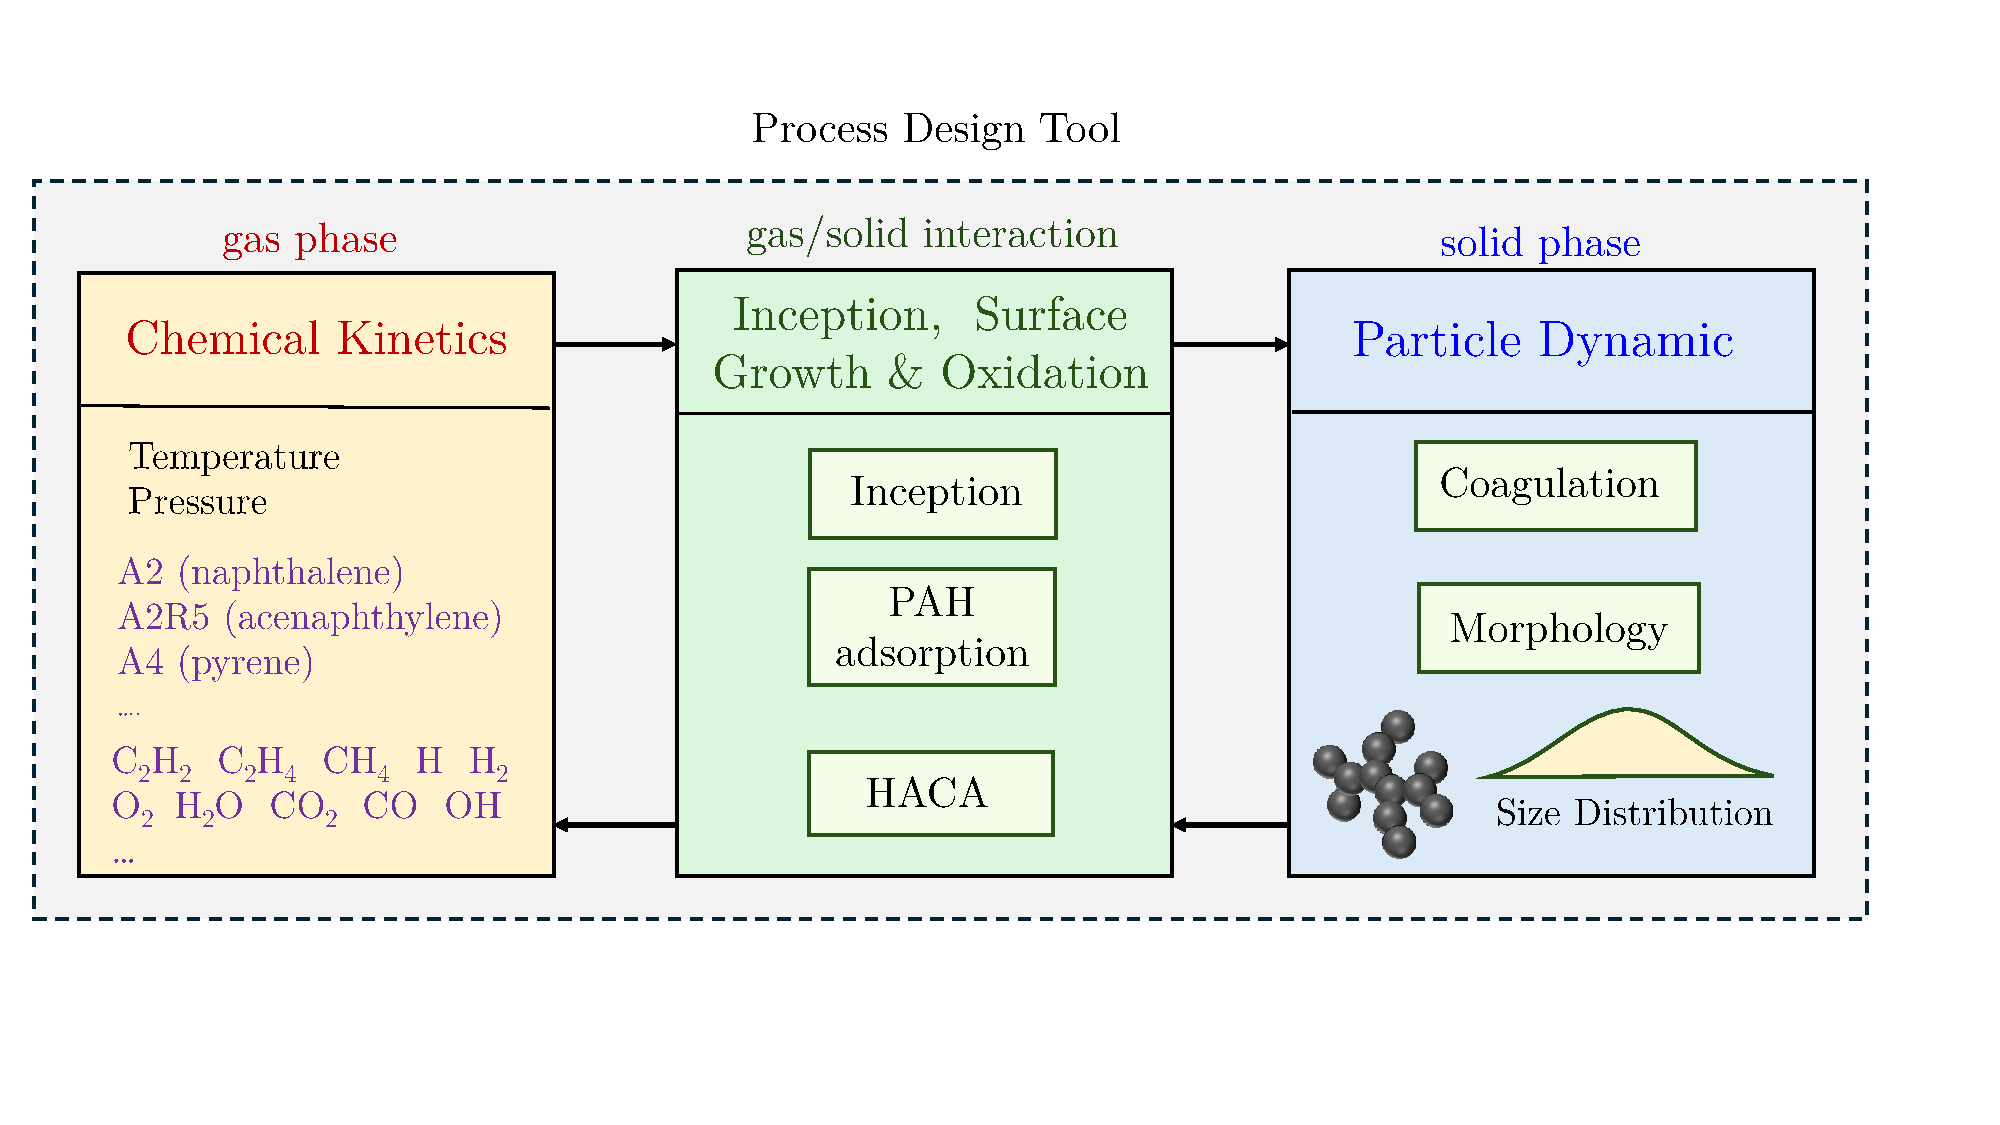
\includegraphics[height=60mm, ]{Figures/Introduction/tooldesign.pdf}
	\caption{The conceptual structure of developed process design tool that account for gas mixture properties, and soot chemistry involving inception, surface growth and oxidation as well as its coagulation leading to the fractal-like morphology}
	\label{fig:tooldesign}
\end{figure}

\section{Research objectives}

The purpose of this project is developing a process design tool to predict soot yield, morphology, composition and size distribution formed in industrial flames and reactors under different temperatures, pressures and residence times. This tool includes a chemical kinetics unit coupled with Cantera~\citep{cantera} to compute thermal and physical properties of gas mixture such as temperature, pressure, density, and enthalpy based on ideal equation of state for the gas mixture. The chemistry of gas mixture is quantified using detail reaction mechanisms that enables tracking concentration of fuel (often $\mathrm{CH_4}$ or $\mathrm{C_2H_4}$ in the context of fundamental soot studies), intermediate species such as $\mathrm{C_2H_2}$ and $\mathrm{H_2}$ essential to surface growth, and PAHs such as benzene (A1), naphthalene (A2) and pyrene (A4) known as building blocks of soot. The second unit accounts for soot inception and surface growth via PAH adsorption and HACA as well as surface oxidation. It accommodates four inception models widely used in literature. The third unit deals with particle dynamics using a MPBM and SPBM to describe the coagulation of soot particles that results in their fractal-like structure with an evolving size distribution. A multi-step validation procedure is followed to assess reliability of each sub-model including collision frequency kernels for particle dynamics models, comparison of predicted agglomerate morphology with DEM results, and finally establishing energy and elemental carbon, and hydrogen balances for all combinations of particle dynamics, inception models and reactors and flames. This tool can be applied to a variety experimental targets with different temperature- and pressure-time-histories, residence times, and fuel compositions.  

As the first step, methane pyrolysis in shock-tube will be simulated using a constant volume reactor. The species measurements will be used to assess the reaction mechanism and examine carbon conversion flux from fuel to smaller intermediates and larger hydrocarbons. The performance of inception models will be analyzed by comparing the predicted soot volume fraction, $f_v$ and primary particle, $d_p$, with data collected from extinction and TEM measurements. A sensitivity analysis will be conducted on model parameters to identify the determining factors that control both $f_v$ and $d_p$ in the framework of shock-tube simulations with short residence time $\approx2$ ms and high temperatures ($\ge 2000$K). Then, the optimization of inception models will be performed by adjusting the rate constants within their physical limit (maximum collision rate of molecules) to minimize the prediction error for yield and morphology. This shows the range of inception flux that enables the model to predict soot yield and morphology represented by $f_v$ and $d_p$, respectively in good agreement with measurements. Then, the optimized rates will be applied to shock-tube in a wide temperature range, and the $f_v$ predictions will be compared with data. A similar investigation will be conducted for flow reactors using plug flow reactor model of omnisoot at lower temperatures and longer residence times  and then the range of expected inception flux with be compared with those of shock-tubes.

% A special attention will be paid to evolving soot refractive index, $m$, absorption function, $E(m)$ with soot morphology and maturity. 


%As discussed before, that enables comparing the performance of implemented inception models applied to various soot-generating targets and careful assessment of their rate constants
%While, this approach can describe inception in low to moderate temperature (<1000 K), and adjusts the inception flux , but it cannot explain how physically-bonded dimers withstand fragmentation at high flame temperatures (>1000 K).      The initial simple The initial PAH classic dimerization describes the inception by physical collision of PAH molecules that  

% 





